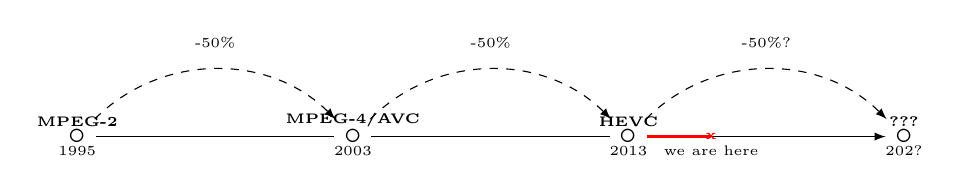
\begin{tikzpicture}[scale=1]
	\def\spacing{3.5}

	\node (mpeg2) at (0,0) {\scalebox{1.25}{$\circ$}};
	\node[above] at (mpeg2) {\tiny \bf MPEG-2};
	\node[below] at (mpeg2) {\tiny 1995};

	\node (mpeg4) at (\spacing,0) {\scalebox{1.25}{$\circ$}};
	\node[above] at (mpeg4) {\tiny \bf MPEG-4/AVC};
	\node[below] at (mpeg4) {\tiny 2003};

	\node (hevc) at (2*\spacing,0) {\scalebox{1.25}{$\circ$}};
	\node[above] at (hevc) {\tiny \bf HEVC};
	\node[below] at (hevc) {\tiny 2013};

	\node (???) at (3*\spacing,0) {\scalebox{1.25}{$\circ$}};
	\node[above] at (???) {\tiny \bf ???};
	\node[below] at (???) {\tiny 202?};

	\draw [-latex] (mpeg2) -- (mpeg4) -- (hevc) -- (???);

	\draw [dashed, -latex] (mpeg2) to [in=135, out=45] (mpeg4);
	\draw [dashed, -latex] (mpeg4) to [in=135, out=45] (hevc);
	\draw [dashed, -latex] (hevc) to [in=135, out=45] (???);

	\node [above] at (\spacing/2,1) {\tiny -50\%};
	\node [above] at (3*\spacing/2,1) {\tiny -50\%};
	\node [above] at (5*\spacing/2,1) {\tiny -50\%?};

	\node[red] (here) at (2.3*\spacing,0) {\tiny \bf x};
	\node[below] at (here) {\tiny we are here};
	\draw [thick,red] (hevc) --++ (3*\spacing/10,0);
\end{tikzpicture}
